\subsection{Background}
Virtual Reality (VR) technology is an area of wearables that have been on the rise
as computer hardware capabilities improve. The Virtual Reality Society defines VR as
a 3D environment generated by a computer that a person can interact with, and be
immersed in such a way that the person can manipulate and interact with the environment
much like they would in \textit{actual} reality \cite{vr_soc_defn}. High-quality
technology and intelligent architectures are required to realize VR due to
the compute-intensive task of processing many inputs and rendering a virtual
world/environment in real time, and depending on the level of detail (LoD), is
an intensive task on its own \cite{hickey_wt4_pres}. Therefore, it is necessary
to make intelligent architecture design decisions to ensure the VR wearable operates
as intended, and with the correct performance specifications.

The most common type of VR wearable is the VR headset, and example is shown below in
Figure \ref{vr:example}. As illustrated, the headset is worn on the head (making it
a wearable), and its screen takes up the user's entire field of view - thereby immersing
them in a virtual environment. Some headsets include audio capabilities and movement
sensors, but this will be discussed later in this section.


\begin{figure}[h]
    \centering
    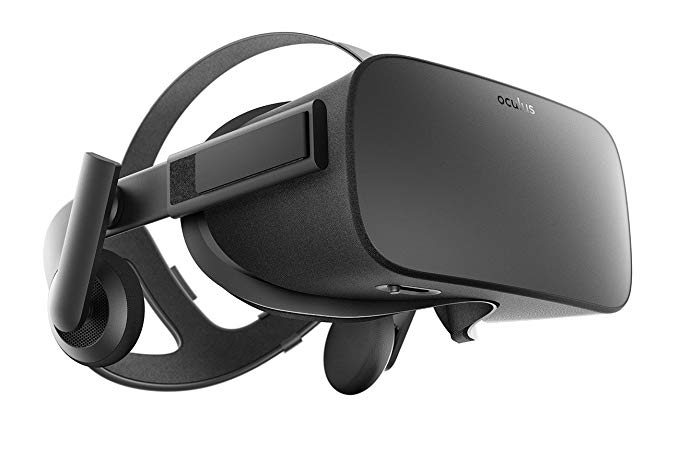
\includegraphics[width=.3\linewidth]{media/vr_headset_example.jpg}
    \caption{Example of archetypal VR headset \cite{vr_headset_pic}}
    \label{vr:example}
\end{figure}

\subsection{Typical Use Cases}
Due to the immersive and potentially high-fidelity rendering that VR can accomplish,
there are several key applications where this technology can be applied. For example, 
VR has the potential for entertainment, business, and medical applications.

\subsubsection{Entertainment}
For entertainment applications, VR has the potential to revolutionize video games.
VR offers the ultimate level of immersion, and allows players to feel as if they
are a part of the world in which they are playing, as shown below in Figure \ref{vr:saber}.
Different VR technologies offer additional peripherals, which can include treadmill-like
surfaces to track players' movements in-game without a controller, and controllers
shaped like gloves that offer haptic feedback when players interact with objects in-game,
thereby taking away elements that limit the immersion of video games \cite{vr_peripherals}.

\begin{figure}[h]
    \centering
    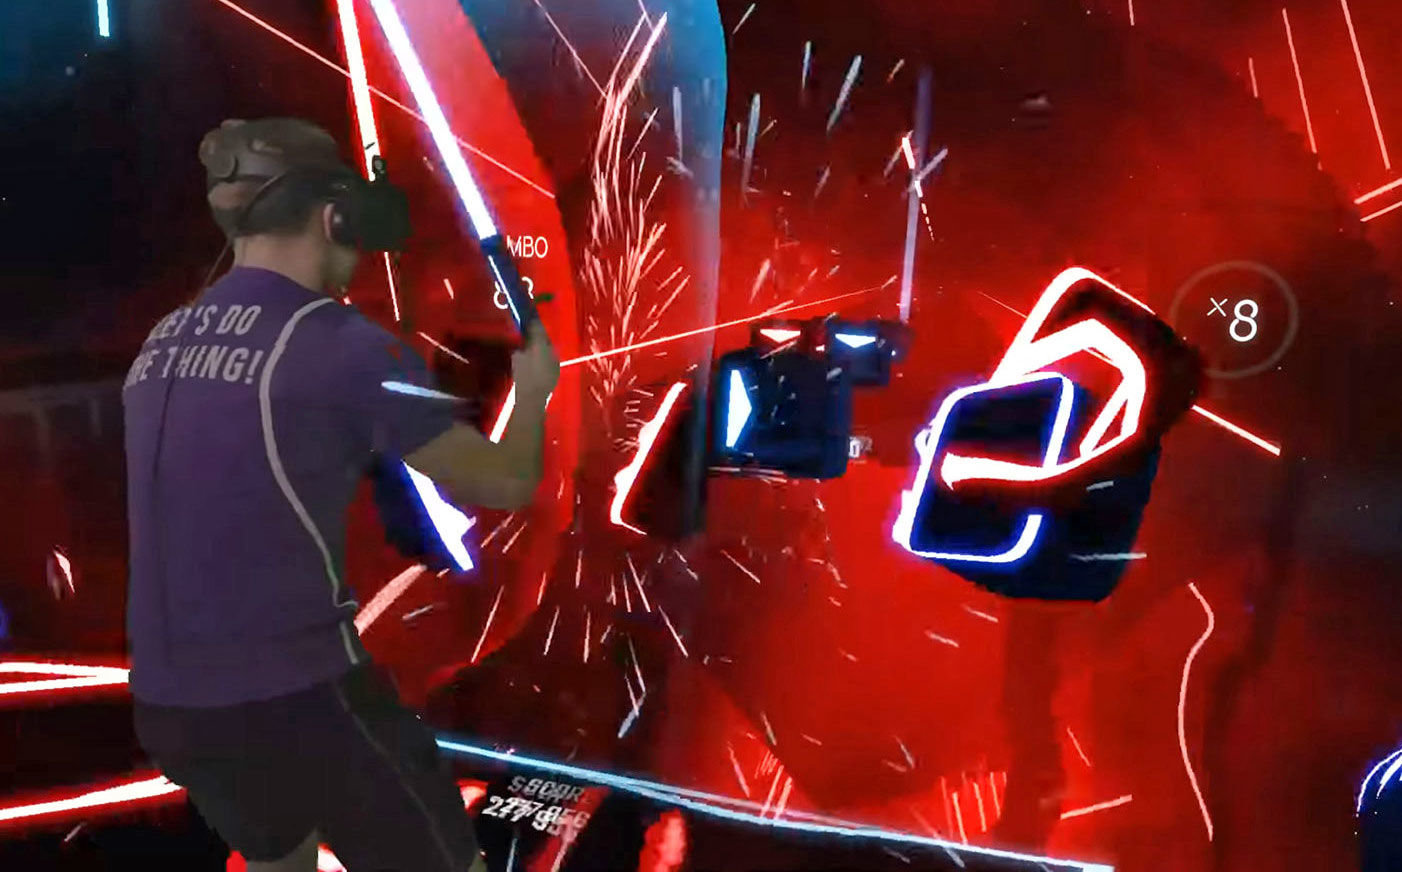
\includegraphics[width=.5\linewidth]{media/beatsaber_vr.jpg}
    \caption{Playing a video game in VR \cite{beatsaber_cite}}
    \label{vr:saber}
\end{figure}

\subsubsection{Business}
For business applications, VR can be used for modelling buildings before they break
ground, but also for completing expensive and dangerous training exercises at a lower
cost, and with zero risk - like ExxonMobil has started doing recently.
Exxon's VR simulator is quite advanced, letting users manipulate the 
virtual world by tracking their head, arm, and leg movements to allow them to 
complete virtual practice work on a model of one of Exxon's real assets \cite{exxon_vr}.
An example of Exxon's setup is shown in Figure \ref{vr:exxon}.
This allows extensive training to be completed with zero consequence of failure and
without having the need to actually send trainees to the platform.

\begin{figure}[h]
    \centering
    \includegraphics[width=.5\linewidth]{media/exxon_vr.jpg}
    \caption{An ExxonMobil employee trains using VR \cite{exxon_vr}}
    \label{vr:exxon}
\end{figure}

\subsubsection{Medical}
For medical applications, VR can be used as both a training tool (shown in
Figure \ref{vr:med_train}), and can allow the opportunity for telepresence 
surgery, where a surgeon can operate on a patient through virtual reality 
from a remote site, while complex machines follow the surgeon's actions 
with acute precision \cite{vr_med_app}. This will allow for doctors to receive
life-like training without having patients going under the knife, and will allow
patients requiring surgery in remote locations to have specialized surgery without the
presence of a specialized surgeon.

\begin{figure}[h!]
    \centering
    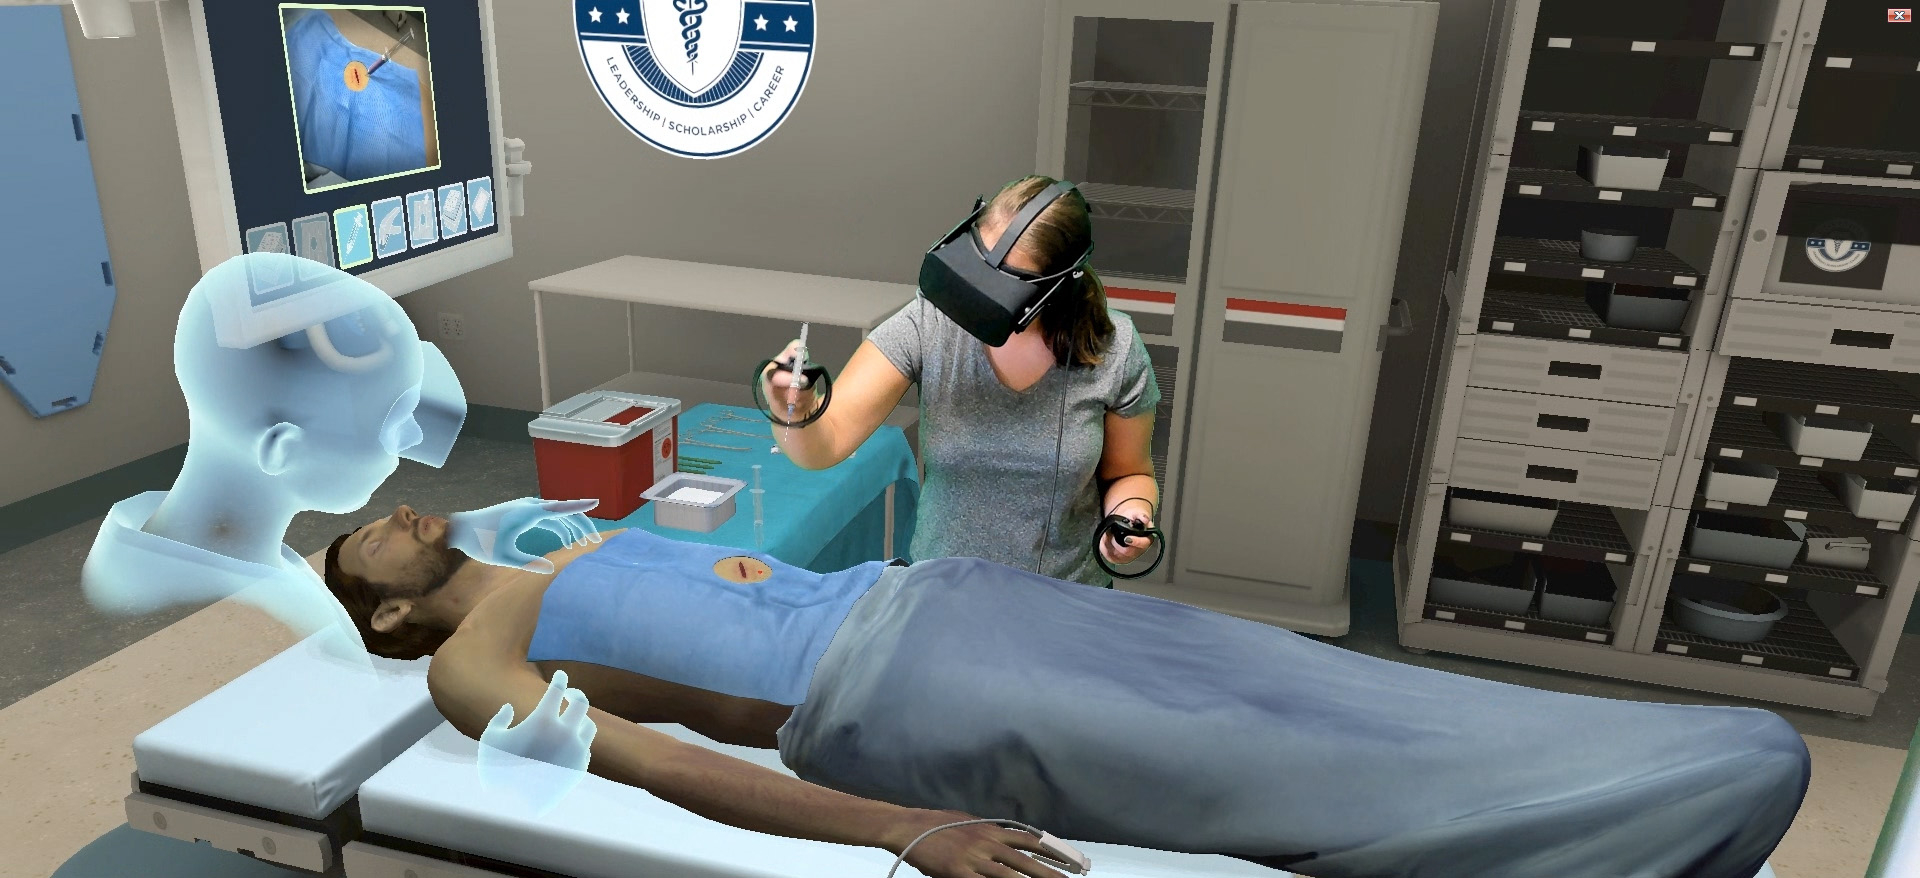
\includegraphics[width=.6\linewidth]{media/med_training_vr.jpg}
    \caption{A surgeon trains using VR \cite{med_train_vr}}
    \label{vr:med_train}
\end{figure}

\subsection{Analysis of Examples}
Two popular examples of virtual reality headsets are the Oculus Quest and the Oculus
Rift S, both shown below in Figure \ref{headsets:pictures}. Much like the two
smartwatches discussed earlier in this report, these two headsets have different
capabilities, which will be discussed later. The pries for these two headsets are listed
below in Table \ref{headset:price} \cite{quest_price} \cite{rift_price}.

% Figure of headsets
\begin{figure}[h]
    \centering
    \begin{subfigure}{.5\textwidth}
      \centering
      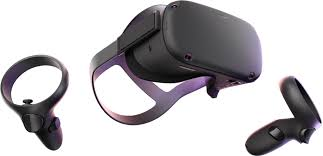
\includegraphics[width=.6\linewidth]{media/oculus_quest.jpg}
      \caption{Oculus Quest VR Headset \cite{quest_headset}}
      \label{head:sub1}
    \end{subfigure}%
    \begin{subfigure}{.5\textwidth}
        \centering
        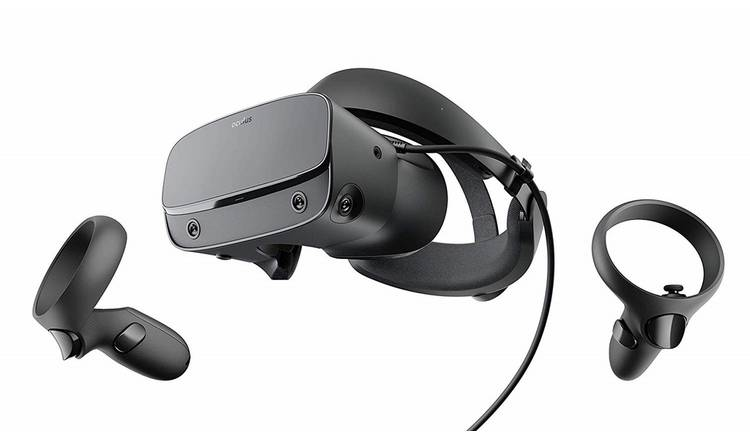
\includegraphics[width=.6\linewidth]{media/oculus_rifts.jpg}
        \caption{Oculus Rift S VR Headset \cite{rift_headset}}
        \label{head:sub2}
      \end{subfigure}
    \caption{VR headsets discussed in this report.}
    \label{headsets:pictures}
\end{figure}

% Headsets prices table
\begin{table}[h]
    \centering
    \caption{Smartwatch Prices}
    \csvautotabular{data/headset_prices.csv} 
    \label{headset:price} 
\end{table}

Even though these two headsets come at the same price, they are targeted at different
market segments, and their architecture reflects that.

\subsubsection{Oculus Quest}
foobar foobar

\subsubsection{Oculus Rift S}
foobar foobar

